%%%%%%%%%%%%%%%%%%%%%%%%%%%%%%%%%%%%%%%%%
% Short Sectioned Assignment
% LaTeX Template
% Version 1.0 (5/5/12)
%
% This template has been downloaded from:
% http://www.LaTeXTemplates.com
%
% Original author:
% Frits Wenneker (http://www.howtotex.com)
%
% License:
% CC BY-NC-SA 3.0 (http://creativecommons.org/licenses/by-nc-sa/3.0/)
%
%%%%%%%%%%%%%%%%%%%%%%%%%%%%%%%%%%%%%%%%%

%----------------------------------------------------------------------------------------
%	PACKAGES AND OTHER DOCUMENT CONFIGURATIONS
%----------------------------------------------------------------------------------------
\documentclass[paper=a4, fontsize=12pt]{scrartcl} % A4 paper and 11pt font size

\usepackage{hyperref}

\usepackage{graphicx} % Required for the inclusion of images
\usepackage{xcolor}

\usepackage[T1]{fontenc} % Use 8-bit encoding that has 256 glyphs
\usepackage{fourier} % Use the Adobe Utopia font for the document - comment this line to return to the LaTeX default
\usepackage[english]{babel} % English language/hyphenation
\usepackage{amsmath,amsfonts,amsthm} % Math packages
\usepackage{listings} % Required for insertion of code
\lstset { %
    language=C++,
    backgroundcolor=\color{black!5}, % set backgroundcolor
    basicstyle=\footnotesize,% basic font setting
}

\usepackage{lipsum} % Used for inserting dummy 'Lorem ipsum' text into the template

\usepackage{sectsty} % Allows customizing section commands
\allsectionsfont{\centering \normalfont\scshape} % Make all sections centered, the default font and small caps

\usepackage{fancyhdr} % Custom headers and footers
\pagestyle{fancyplain} % Makes all pages in the document conform to the custom headers and footers
\fancyhead{} % No page header - if you want one, create it in the same way as the footers below
\fancyfoot[L]{} % Empty left footer
\fancyfoot[C]{} % Empty center footer
\fancyfoot[R]{\thepage} % Page numbering for right footer
\renewcommand{\headrulewidth}{0pt} % Remove header underlines
\renewcommand{\footrulewidth}{0pt} % Remove footer underlines
\setlength{\headheight}{13.6pt} % Customize the height of the header

\numberwithin{equation}{section} % Number equations within sections (i.e. 1.1, 1.2, 2.1, 2.2 instead of 1, 2, 3, 4)
\numberwithin{figure}{section} % Number figures within sections (i.e. 1.1, 1.2, 2.1, 2.2 instead of 1, 2, 3, 4)
\numberwithin{table}{section} % Number tables within sections (i.e. 1.1, 1.2, 2.1, 2.2 instead of 1, 2, 3, 4)

\setlength\parindent{0pt} % Removes all indentation from paragraphs - comment this line for an assignment with lots of text

%----------------------------------------------------------------------------------------
%	TITLE SECTION
%----------------------------------------------------------------------------------------

\newcommand{\horrule}[1]{\rule{\linewidth}{#1}} % Create horizontal rule command with 1 argument of height

\title{	
\normalfont \normalsize 
\textsc{Georgia Institute of Technology, ECE} \\ [25pt] % Your university, school and/or department name(s)
\horrule{0.5pt} \\[0.4cm] % Thin top horizontal rule
\huge RED vs DropTail \\ % The assignment title
\horrule{2pt} \\[0.5cm] % Thick bottom horizontal rule
}

\author{Arunprasanna Sundararajan Poorna} % Your name

\date{\normalsize\today} % Today's date or a custom date

\begin{document}

\maketitle 

% Print the title
%----------------------------------------------------------------------------------------
%	PROBLEM 1
%----------------------------------------------------------------------------------------
%\center {GTID: 903062365\newline}
\begin{center}
\href{mailto:asp6@gatech.edu}{\hspace{92pt}asp6@gatech.edu\newline}
\hspace{92pt}{ECE 6110\newline}
\hspace{88pt}{Spring 2015}
\end{center}

\vspace{60pt}
\section{Introduction}
%\lipsum[2] % Dummy text
%
%\begin{align} 
%\begin{split}
%(x+y)^3 	&= (x+y)^2(x+y)\\
%&=(x^2+2xy+y^2)(x+y)\\
%&=(x^3+2x^2y+xy^2) + (x^2y+2xy^2+y^3)\\
%&=x^3+3x^2y+3xy^2+y^3
%\end{split}					
%\end{align}
High-speed Networks with large delay bandwidth products are prevalent today. TCP congestion avoidance deals with managing congestion by ensuring queues do not fill up. We need mechanisms to ensure queue management while maintaining a high throughput. In this report we will see some of the results of our simulation of two popular queue management techniques: RED and DropTail. 
%------------------------------------------------
\newpage
\subsection{Topology}

\begin{figure}[h]
\begin{center}
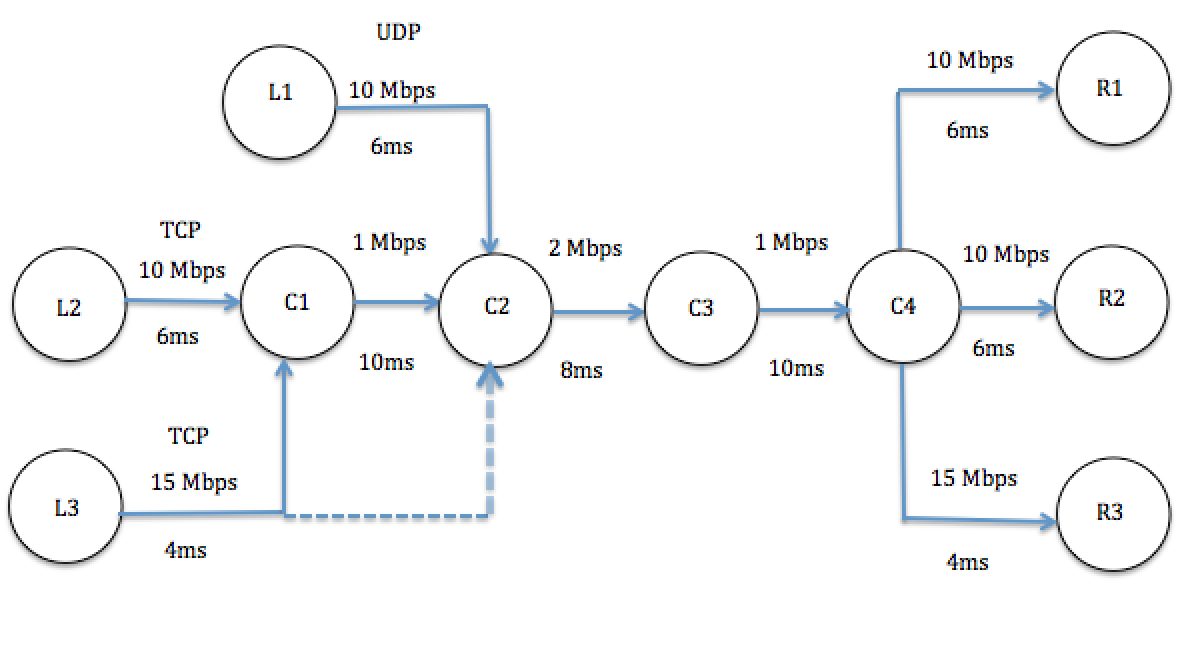
\includegraphics[width=1.02\textwidth]{1} % Include the image placeholder.png
\caption{Topology of the Simulation Environment}
\end{center}
\end{figure}
\vspace{-40pt}
\paragraph{The Topology}
that we have simulated is shown above. Each link is defined by it's capacity and the speed of light delay. We have constructed a non-trivial topology that has more than a single bottleneck link. This makes for more interesting observations on whether TCP congestion avoidance performs well or not when competing with a UDP Flow that is hogging (or not hogging!) the bottleneck. The dashed lines represent an alternate topology used to see difference in results, some of which have been discussed below.
\paragraph{Assumptions\newline}
\hspace{-10pt}*Receiver windows do not restrict the flows(they are large). \newline
*The load is constant for each simulation run.\newline
*TCP1 has a slightly larger bandwidth-delay product than TCP2\newline
*UDP has been implemented using on-off application in ns3. It is the change in UDP flow that results in the change of load on network.

\paragraph{A Mix of TCP and UDP Flows}have been used. We are interested in seeing how UDP flows affect when competing with TCP flows and their congestion avoidance schemes. I have varied the rate of transmission of UDP Flows(load) and repeated experiments to notice the effect of the UDP flow on the bottleneck link. We have not implemented simultaneous use of DropTail and RED in this simulation. We have only simulated them separately.

%------------------------------------------------

\newpage
\subsection{Background}

\paragraph{\newline How does DropTail Work?\newline} 
\hspace{-10pt} DropTail works by dropping packets if the queue length exceeds a certain\emph{ drop level} with a fixed\emph{ drop probability}. Drop Tail gateways result in global synchronization in the network. Packets are dropped from several connections and their windows decrease at the same time affecting the throughput. Implementing FIFO queues also results in "lock-outs" in which a small subset of flows with a higher rate can result in performance issues for flows with lower rates of packet transmission. 

\paragraph{ What do we Expect from RED?\newline} 
\hspace{-10pt}RED performs congestion avoidance by controlling the average queue size and successfully avoids the global synchronization problem we faced with fixed drop probability in DropTail. RED also results in more efficient local and global use of network resources by reducing packet losses that occur when queues overflow. RED uses a random factor in selecting which packets to drop thus avoiding "flow outs". 

%----------------------------------------------------------------------------------------
%	PROBLEM 2
%----------------------------------------------------------------------------------------

\section{Performance Expectations}

%------------------------------------------------

\subsection{Parameters and their Expected Change}
\begin{itemize}
	\item DropTail  
		\begin{itemize}
		\item Queue length threshold
			\begin{itemize}
			\item Packets are dropped with a fixed probability after threshold.\newline
			\end{itemize}
		\end{itemize}
	\item RED
		\begin{itemize}
		\item Minimum Threshold (max\textsubscript{th})
			\begin{itemize}
			\item Queue length threshold for triggering probabilistic drops.
			\end{itemize}
		\item Maximum Threshold (min\textsubscript{th})
			\begin{itemize}
			\item Queue length threshold for triggering forced drops. 
			\end{itemize}
		\item  W\textsubscript{f}
			\begin{itemize}
			\item Weighting Factor for Average Queue length computation.
			\end{itemize}
		\item Queue Length 
			\begin{itemize}
			\item The maximum number of packets that can be enqueued.
			\item We expect throughput to increase with increase in queue length.
			\end{itemize}
		\item max\textsubscript{p}
			\begin{itemize}
			\item Maximum Probability of performing an early drop.\newline
			\end{itemize}
		\end{itemize}
	
	\item Load
		\begin{itemize}
		\item The Traffic Load 
			\begin{itemize}
			\item The traffic load was varied by varying the UDP rate (by varying \emph{duty cycle} of on-off application).
			\item The bottleneck ensures that TCP utilization/throughput depends on the above traffic, since UDP is a connectionless protocol.
			\end{itemize}
		\end{itemize}
	\item Receiver Window Size
		\begin{itemize}
		\item Receiver Window Size TCP connection
			\begin{itemize}
			\item We expect that throughput increases with increase in receiver window size.
			\item Assuming, that the bottleneck can handle the traffic.
			\end{itemize}
		\end{itemize}
\end{itemize}

%------------------------------------------------


\section{Graphs and Results}
%\lipsum[2] % Dummy text
%
%\begin{align} 
%\begin{split}
%(x+y)^3 	&= (x+y)^2(x+y)\\
%&=(x^2+2xy+y^2)(x+y)\\
%&=(x^3+2x^2y+xy^2) + (x^2y+2xy^2+y^3)\\
%&=x^3+3x^2y+3xy^2+y^3
%\end{split}					
%\end{align}


%------------------------------------------------
Let us discuss the results we obtained by analysis of graphs and reasoning the behavior behind these graphs. This section is organized into different sub sections containing different graphs showcasing different trends.

\subsection{Varying Queue Length of DropTail}
\begin{figure}[h]
\begin{center}$
\begin{array}{cccc}
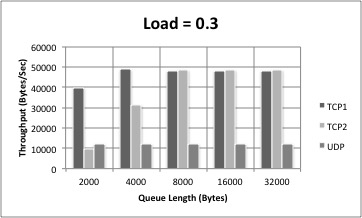
\includegraphics[trim={.1cm 0.1cm 0.1cm 1.1cm},clip, width=3.0in, height=2.2in]{Q3.png} &
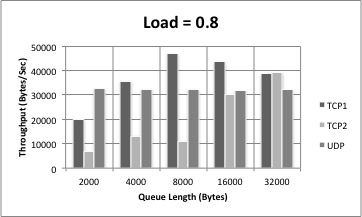
\includegraphics[trim={0.1cm 0.1cm 0.1cm 1.1cm},clip,width=3.0in, height=2.2in]{Q8.png}  &
\end{array}$
\end{center}
\vspace{-20pt}
%\caption{Throughput of flows for varying queue length}
%\caption{Throughput of three flows for varying queue lengths}
\caption{Throughput of three flows for varying queue lengths and load factors of 0.25 and 0.5}
\end{figure}
\begin{figure}[h]
\begin{center}$
\begin{array}{c}
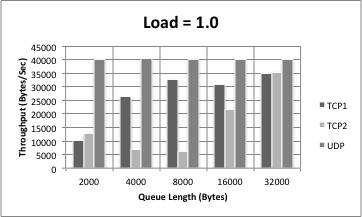
\includegraphics[trim={0,1cm 0.1cm 0.1cm 1.1cm},clip,width=3.0in,height=2.2in]{Q1.png} 
\end{array}$
\end{center}
\caption{Throughput of three flows for varying queue lengths and load factor of 0.75}
\end{figure}
\newpage
\paragraph{\newline The Story Behind the Graphs} 
\hspace{-10pt}\paragraph{Figure 3.1}
\hspace{-10pt} shows how the throughput of the three flows differs when the three competing flows use DropTail and the Queue length threshold of DropTail is varied. We can clearly see that as the load is increased the UDP connection strangles the other two TCP connections. Load factor of 0.5 shows us interesting trends. We can see a reversal at queue length of 8000 bytes. That is, the TCP connection with lower bandwidth gets a higher throughput. Although counterintuitive, this makes sense since DropTail kills the TCP connection with a higher rate. We explained this phenomenon in our background study.
\paragraph{Figure 3.2}
\hspace{-10pt} shows the throughput of three flows for a congested network where the UDP connection has a higher on-off rate, thus making the two TCP connections suffer. This is a consistent phenomenon observed for all experiments conducted. The connectionless protocol blasts away while the cautious TCP suffers from low throughput. We can also observe that the sum total goodput of all three flows increases as queue length increases.
\newpage
\subsection{Varying Minimum Threshold of RED}
\begin{figure}[ht]
\begin{center}$
\begin{array}{cccc}
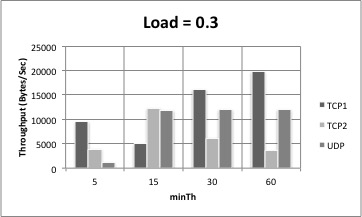
\includegraphics[trim={0.1cm 0.1cm 0.1cm 1.1cm},clip,width=3.0in, height=2.2in]{MI3.png} &
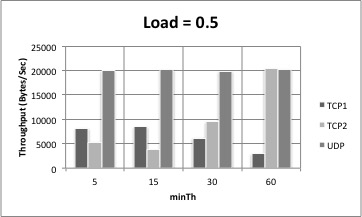
\includegraphics[trim={0.1cm 0.1cm 0.1cm 1.1cm},clip,width=3.0in, height=2.2in]{MI5.png}  &
\end{array}$
\end{center}
\caption{Throughput of three flows for Minimum Threshold and load factors of 0.25 and 0.5}
\end{figure}
\begin{figure}[h]
\vspace{-20pt}
\begin{center}$
\begin{array}{cccc}
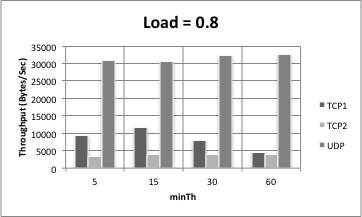
\includegraphics[trim={0.1cm 0.1cm 0.1cm 1.1cm},clip,width=3.0in, height=2.2in]{MI8.png} 
\end{array}$
\end{center}
\caption{Throughput of three flows for Minimum Threshold and load factor of 0.75}
\end{figure}

\paragraph{The Story Behind the Graphs\newline} 
\hspace{-10pt}Figure 3.3 and 3.4 show the variation as the minimum threshold is increased for different load factors. We can see that UDP connection saturates at a load of 0.5 itself. Load of 0.25 gives us interesting trends. We can see that UDP throughput increases consistently and that TCP1 which has higher bandwidth performs well only at a minimum \emph{minimum threshold}. This is as expected since a very low threshold lets RED make probabilistic drops at lower thresholds. 
\newpage
\subsection{Varying Maximum Threshold of RED}
\begin{figure}[h]
\begin{center}$
\begin{array}{cccc}
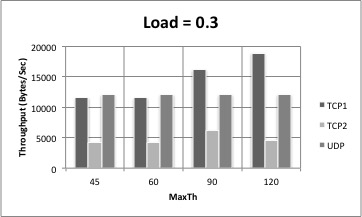
\includegraphics[trim={0.1cm 0.1cm 0.1cm 1.1cm},clip,width=3.0in, height=2.2in]{MA3.png} &
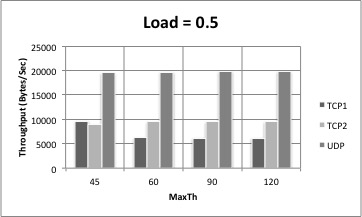
\includegraphics[trim={0.1cm 0.1cm 0.1cm 1.1cm},clip,width=3.0in, height=2.2in]{MA5.png}  &
\end{array}$
\end{center}
\vspace{-20pt}
%\caption{Throughput of flows for varying queue length}
\caption{Throughput of three flows for Maximum Threshold and load factors of 0.25 and 0.5}
\end{figure}
\vspace{25pt}
\begin{figure}[h]
\vspace{-40pt}
\begin{center}$
\begin{array}{cccc}
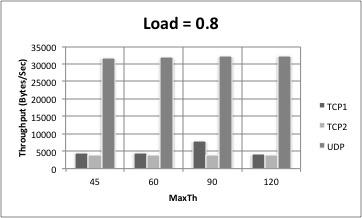
\includegraphics[trim={0.1cm 0.1cm 0.1cm 1.1cm},clip,width=3.0in, height=2.2in]{MA8.png} 
\end{array}$
\end{center}
\caption{Throughput of three flows for Maximum Threshold and load factor of 0.75}
\end{figure}

\paragraph{The Story Behind the Graphs} 
\paragraph{Figure 3.5}
\hspace{-10pt} (the first graph) is of interest to us. We can see that TCP1 now dominates more and more as we increase the maximum threshold. This is because as we increase the maximum threshold, we make lesser and lesser forced drops! This let's TCP connections with higher bandwidth perform well. RED is fair in this regard, since the drop probability depends on the rate at which TCP connections send data. This gives an unfair advantage to UDP though, since it is a connectionless protocol. We can see that when the difference between min\textsubscript{th} and max\textsubscript{th} is higher, the total goodput of three flows is higher, since the forced drops are lesser. 

\newpage

\subsection{Varying Weighting Factor of RED}
\begin{figure}[h]
\begin{center}$
\begin{array}{cccc}
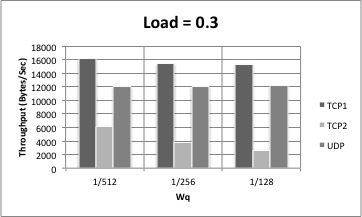
\includegraphics[trim={0.1cm 0.1cm 0.1cm 1.1cm},clip,width=3.0in, height=2.2in]{WQ3.png} &
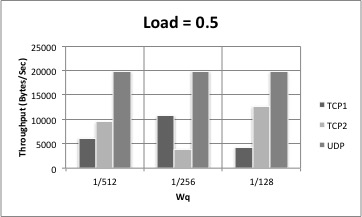
\includegraphics[trim={0.1cm 0.1cm 0.1cm 1.1cm},clip,width=3.0in, height=2.2in]{WQ5.png}  &
\end{array}$
\caption{Throughput of three flows for varying Weighting factors and load factors of 0.25 and 0.5}
\end{center}
\vspace{-20pt}
%\caption{Throughput of flows for varying queue length}
\end{figure}



\paragraph{The Story Behind the Graphs} 
\paragraph{Figure 3.7}
\hspace{-10pt} shows us our most important takeaway about RED. RED is incredibly difficult to tune and optimize. We can see that actual performance of different flows depends on how the weighing factor is set. We can also see that it is load dependent. Thus, a static value of weighing factor cannot be used to optimize connections. This is one of the major reasons why using RED is not as easy as it's design philosophy makes it out to be.
\newpage
\subsection{Varying Maximum Probability of Random Drop}
\begin{figure}[h]
\begin{center}$
\begin{array}{cccc}
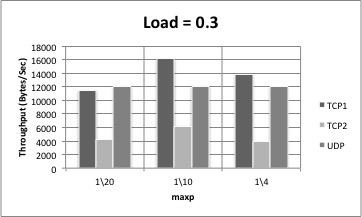
\includegraphics[trim={0.1cm 0.1cm 0.1cm 1.1cm},clip,width=3.0in, height=2.2in]{MP3.png} &
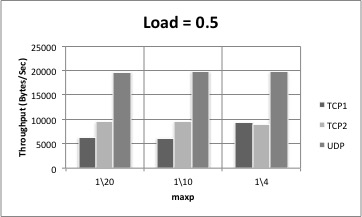
\includegraphics[trim={0.1cm 0.1cm 0.1cm 1.1cm},clip,width=3.0in, height=2.2in]{MP5.png}  &
\end{array}$
\end{center}
\vspace{-20pt}
%\caption{Throughput of flows for varying queue length}
\end{figure}
\vspace{25pt}
\begin{figure}[h]
\vspace{-40pt}
\begin{center}$
\begin{array}{cccc}
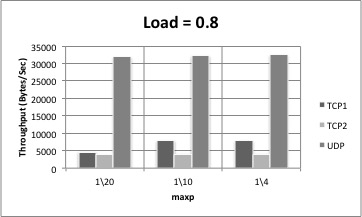
\includegraphics[trim={0.1cm 0.1cm 0.1cm 1.1cm},clip,width=3.0in, height=2.2in]{MP8.png} 
\end{array}$
\end{center}
\caption{Throughput of three flows for Varying Maximum Probability and load factors of .25, .5 and .75}
\end{figure}

\paragraph{The Story Behind the Graphs} 
\paragraph{Figure 3.8}
\hspace{-10pt} shows us that as max\textsubscript{p} increases, the total throughput (added throughput of all three flows decreases). The paper \emph{Tuning RED for Web Traffic} claims that longer flows are affected more by changing w\textsubscript{f} and max\textsubscript{p}. This is not evident from the topology we have selected. A more non uniform and realistic topology is required to observe this clearly. I did try to shift the TCP nodes away from each other(\emph{as shown in the alternate topology}). But it did not result in any concrete trend. Max\textsubscript{p} and w\textsubscript{f} have been difficult to set, to observe the trends shown in the paper.

 \newpage
\section{Conclusion}

\paragraph{What Did we Learn?\newline\newline}
\hspace{-10pt}
We started out with curiosity about whether RED was as beneficial as it's design claimed it to be. The most important and recurring theme in our experiments has been that RED is difficult to configure. Thus, obtaining good results with it is difficult albeit possible.These "optimal" settings were non obvious and were arrived at through a trial and error process. This drawback of requiring a trained network administrator constantly ensuring that RED performs well is a serious blow against using RED large scale. We did notice that a well configured RED performed well, especially under higher loads when packets were more likely to be dropped due to congestion. A properly configured DropTail FIFO queue may suffice to help us avoid congestion under these circumstances. It's performance issues can be dealt with by minor optimizations wherever possible and we can keep the threshold fairly high to ensure that it does not interfere with the network's operation extensively.
\section{Appendix}
\subsection{NS3 Code}
\lstset {language=C++}
\begin{lstlisting}
//include necessary ns3 modules
#include "ns3/core-module.h"
#include "ns3/network-module.h"
#include "ns3/internet-module.h"
#include "ns3/point-to-point-module.h"
#include "ns3/random-variable-stream.h"
#include "ns3/applications-module.h"
#include "ns3/packet-sink-helper.h"
#include "ns3/uinteger.h"
#include "ns3/point-to-point-dumbbell.h"
#include "ns3/drop-tail-queue.h"
#include "ns3/constant-position-mobility-model.h"
#include "ns3/test.h"

using namespace ns3;

int main (int argc, char *argv[])
{
//std::cout << "\n Running Simulation " << std::endl;
Time::SetResolution (Time::NS);
std::string queueType = "DropTail";
//initialize all parameters used
int nodes = 0; 
int window_size = 4000; 
int maxBytes = 1000000;
int qlen = 800;
double minimum_threshold = 50.0;
double maximum_threshold = 150.0;
double Wq = 1.0/100.0;
double maxP = 1.0/10.0;
double load = 0.75;
//debug mode
#ifdef DEBUG
std::cout<< "\nDEBUG MODE ON" <<std::endl;
#endif

//get command line arguments if they've been given
CommandLine cmd;
cmd.AddValue ("window_size", "TCP Receiver window size", window_size);
cmd.AddValue ("maxBytes", "Max bytes that can be sent", maxBytes);
cmd.AddValue ("minTh", "Min threshold for prob drops", minimum_threshold);
cmd.AddValue ("maximum_threshold", "Max threshold for problitistic drops", 
maximum_threshold);
cmd.AddValue ("maxP", "Max probability of doing an early drop", maxP);
cmd.AddValue ("Wq", "Weighting factor for average queue length computation", Wq);
cmd.AddValue ("qlen", "Maximum number of bytes that can be enqueued", qlen);
cmd.AddValue ("load", "Load", load);
cmd.Parse(argc, argv);
#ifdef DEBUG
{
	std::cout << "\nInput values" << std::endl;
std::cerr << "queueType = " << queueType << "\n"<< "load=" << load << "\n"
<< "window_size=" << window_size << "\n"<< "maxBytes=" << maxBytes << "\n"
<< "\tminimum_threshold=" << minimum_threshold << "\n"<< "\tmaximum_threshold=" 
<< maximum_threshold << "\n"
<< "\tmaxP=" << maxP << "\n"<< "\tWq=" << Wq << "\n"<< "\tqueue_length=" 
<< qlen << "\n"<< std::endl;
}	
#endif
//set configuration for DropTailQueue, RedQUeue and TCPSocket
Config::SetDefault ("ns3::DropTailQueue::Mode", 
EnumValue(DropTailQueue::QUEUE_MODE_BYTES));
Config::SetDefault ("ns3::DropTailQueue::MaxBytes", UintegerValue(maxBytes));
Config::SetDefault ("ns3::RedQueue::Mode", 
EnumValue (RedQueue::QUEUE_MODE_BYTES));
Config::SetDefault ("ns3::RedQueue::MinTh", DoubleValue (minimum_threshold));
Config::SetDefault ("ns3::RedQueue::MaxTh", DoubleValue (maximum_threshold));
Config::SetDefault ("ns3::RedQueue::QW", DoubleValue (Wq));
Config::SetDefault ("ns3::RedQueue::QueueLimit", UintegerValue (qlen));
Config::SetDefault ("ns3::RedQueue::LInterm", DoubleValue (maxP));
Config::SetDefault ("ns3::TcpSocket::RcvBufSize", UintegerValue(window_size));


std::string type;//define a string
type = "ns3::RedQueue"; //change to DropTailQueue if needed

NodeContainer n;
//number of nodes we are going to create. Max is just 10 in our topology.
nodes=12;
n.Create(nodes);

//define topology by defining the links for nodes created
//change this below to obtain different topologies discussed in the report
NodeContainer bottleneck_link_1 = NodeContainer(n.Get(0), n.Get(1));
NodeContainer bottleneck_link_3 = NodeContainer(n.Get(1), n.Get(2));
NodeContainer bottleneck_link_2 = NodeContainer(n.Get(0), n.Get(3));
NodeContainer source_1 = NodeContainer(n.Get(3), n.Get(4));
NodeContainer source_2 = NodeContainer(n.Get(3), n.Get(5));
NodeContainer source_3 = NodeContainer(n.Get(3), n.Get(6));
NodeContainer sink_1 = NodeContainer(n.Get(2), n.Get(7));
NodeContainer sink_2 = NodeContainer(n.Get(2), n.Get(8));
NodeContainer sink_3 = NodeContainer(n.Get(2), n.Get(9));

//define the router nodes 
NodeContainer routerNodes;
routerNodes.Add(n.Get(0));
routerNodes.Add(n.Get(1));
routerNodes.Add(n.Get(2));
routerNodes.Add(n.Get(3));


//define the left nodes that act as source
NodeContainer leftNodes;
leftNodes.Add(n.Get(4));
leftNodes.Add(n.Get(5));
leftNodes.Add(n.Get(6));

//define the right nodes that act as sink
NodeContainer rightNodes;
rightNodes.Add(n.Get(7));
rightNodes.Add(n.Get(8));
rightNodes.Add(n.Get(9));

//call point to point helper to set bandwidth and speed of
 light delay and specify type of queue management!
PointToPointHelper bottleneck1;
bottleneck1.SetDeviceAttribute ("DataRate", StringValue ("1Mbps"));
bottleneck1.SetChannelAttribute ("Delay", StringValue ("10ms"));
bottleneck1.SetQueue (type);
NetDeviceContainer device_bottleneck_link_2 = bottleneck1.Install(bottleneck_link_2);

PointToPointHelper bottleneck2;
bottleneck2.SetDeviceAttribute ("DataRate", StringValue ("1Mbps"));
bottleneck2.SetChannelAttribute ("Delay", StringValue ("10ms"));
bottleneck2.SetQueue (type);
NetDeviceContainer device_bottleneck_link_3 = bottleneck2.Install(bottleneck_link_3);

PointToPointHelper center;
center.SetDeviceAttribute ("DataRate", StringValue ("1Mbps"));
center.SetChannelAttribute ("Delay", StringValue ("10ms"));
NetDeviceContainer device_bottleneck_link_1 = center.Install(bottleneck_link_1);

PointToPointHelper p2pLeft;
p2pLeft.SetDeviceAttribute ("DataRate", StringValue ("10Mbps"));
p2pLeft.SetChannelAttribute ("Delay", StringValue ("6ms"));
NetDeviceContainer device_source_1 = p2pLeft.Install(source_1);

PointToPointHelper p2pLeft2;
p2pLeft2.SetDeviceAttribute ("DataRate", StringValue ("10Mbps"));
p2pLeft2.SetChannelAttribute ("Delay", StringValue ("6ms"));
NetDeviceContainer device_source_2 = p2pLeft2.Install(source_2);
//give the other TCP connection more bandwidth to get varied results
PointToPointHelper p2pLeft3;
p2pLeft3.SetDeviceAttribute ("DataRate", StringValue ("15Mbps"));
p2pLeft3.SetChannelAttribute ("Delay", StringValue ("4ms"));
NetDeviceContainer device_source_3 = p2pLeft3.Install(source_3);

PointToPointHelper p2pRight;
p2pRight.SetDeviceAttribute ("DataRate", StringValue ("10Mbps"));
p2pRight.SetChannelAttribute ("Delay", StringValue ("6ms"));
NetDeviceContainer device_sink_1 = p2pRight.Install(sink_1);

PointToPointHelper p2pRight2;
p2pRight2.SetDeviceAttribute ("DataRate", StringValue ("10Mbps"));
p2pRight2.SetChannelAttribute ("Delay", StringValue ("6ms"));
NetDeviceContainer device_sink_2 = p2pRight2.Install(sink_2);

PointToPointHelper p2pRight3;
p2pRight3.SetDeviceAttribute ("DataRate", StringValue ("15Mbps"));
p2pRight3.SetChannelAttribute ("Delay", StringValue ("4ms"));
NetDeviceContainer device_sink_3 = p2pRight3.Install(sink_3);

NetDeviceContainer array_of_devices[] = {device_bottleneck_link_2, 
device_bottleneck_link_3, device_bottleneck_link_1, device_source_1, 
device_source_2, device_source_3, device_sink_1, device_sink_2, device_sink_3};
std::vector<NetDeviceContainer> devices(array_of_devices,
 array_of_devices + sizeof(array_of_devices) / sizeof(NetDeviceContainer));
//install the internet stack using the internetstackhelper
InternetStackHelper stack;
stack.Install (n);

//create the IP addresses required and give it the same subnet mask as required
Ipv4AddressHelper ipv4;
std::vector<Ipv4InterfaceContainer> ifaceLinks(nodes-1);
for(uint32_t i=0; i<devices.size(); ++i)
 {
std::ostringstream sub_net;
sub_net << "192.10." << i+1 << ".0";
ipv4.SetBase(sub_net.str().c_str(), "255.255.255.0");
ifaceLinks[i] = ipv4.Assign(devices[i]);
}
//define min bandwidth
double min_bandwidth = 1000000;
// define duty cycle and determine rate of on-off application
double duty_cycle = 0.5;
uint64_t rate = (uint64_t)(load*min_bandwidth / 3 / duty_cycle); 

//define a random port
int port_number = 12;
 //set UDP to on off application and determine it using the rate calculated above
OnOffHelper onOffUdp1("ns3::UdpSocketFactory", 
Address(InetSocketAddress(ifaceLinks[6].GetAddress(1), port_number)));
onOffUdp1.SetConstantRate(DataRate(rate));
onOffUdp1.SetAttribute("OnTime", StringValue("ns3::ConstantRandomVariable
[Constant=0.5]"));
onOffUdp1.SetAttribute("OffTime", StringValue("ns3::ConstantRandomVariable[
Constant=0.5]"));


//I have used Bulksendhelper for TCP connections. UDP connection 
load suffices to provide us trends on a congested network.
BulkSendHelper source1 ("ns3::TcpSocketFactory",
 InetSocketAddress(ifaceLinks[7].GetAddress(1), port_number));
source1.SetAttribute("MaxBytes", UintegerValue (maxBytes));

BulkSendHelper source2 ("ns3::TcpSocketFactory", 
InetSocketAddress(ifaceLinks[8].GetAddress(1), port_number));
source2.SetAttribute("MaxBytes", UintegerValue (maxBytes));

ApplicationContainer sourceApps;
//define the sources and start them
sourceApps.Add(source1.Install(source_2.Get(1)));
sourceApps.Add(source2.Install(source_3.Get(1)));
sourceApps.Add(onOffUdp1.Install(source_1.Get(1)));
sourceApps.Start(Seconds(0.0));
sourceApps.Stop(Seconds(15.0));
//define the sinks
PacketSinkHelper sinkUdp1("ns3::UdpSocketFactory",
Address(InetSocketAddress(Ipv4Address::GetAny(), port_number)));

PacketSinkHelper sinkTcp1("ns3::TcpSocketFactory",
Address(InetSocketAddress(Ipv4Address::GetAny(), port_number)));

PacketSinkHelper sinkTcp2("ns3::TcpSocketFactory",
Address(InetSocketAddress(Ipv4Address::GetAny(), port_number)));

ApplicationContainer sinkApps;
sinkApps.Add(sinkTcp1.Install(sink_2.Get(1)));
sinkApps.Add(sinkTcp2.Install(sink_3.Get(1)));
sinkApps.Add(sinkUdp1.Install(sink_1.Get(1)));
//sink has same start and end time as source
sinkApps.Start(Seconds(0.0));
sinkApps.Stop(Seconds(15.0));

//dont forget to populate the routing tables!
Ipv4GlobalRoutingHelper::PopulateRoutingTables ();

Simulator::Stop (Seconds (15.0));
Simulator::Run ();

std::vector<int> goodputs;
int i = 0;
//Iterate through the flows
for(ApplicationContainer::Iterator ii = sinkApps.Begin(); ii != sinkApps.End(); ++ii)
 {
Ptr<PacketSink> sink = DynamicCast<PacketSink> (*ii);
int bytes_received = sink->GetTotalRx ();//get total bytes received
goodputs.push_back(bytes_received / 15.0);//total bytes divided by time
if(i==0)
{
std::cout << "\nTCP1 :" << std::endl;
std::cout << "\tTotal Bytes Received: " << bytes_received << std::endl;
std::cout << "\tGoodput: " << goodputs.back() << " Bytes/seconds" << std::endl;
}
if(i==1)
{
std::cout << "\nTCP2 :" << std::endl;
std::cout << "\tTotal Bytes Received: " << bytes_received << std::endl;
std::cout << "\tGoodput: " << goodputs.back() << " Bytes/seconds" << std::endl;
}
if(i==2)
{
std::cout << "\nUDP:" << std::endl;
std::cout << "\tTotal Bytes Received: " << bytes_received << std::endl;
std::cout << "\tGoodput: " << goodputs.back() << " Bytes/seconds" << std::endl;
}
++i;
}

std::cout << "\nIt worked!" << std::endl;
std::cerr << "queueType = " << queueType << "\n"<< "load=" << load << "\n"
<< "window_size=" << window_size << "\n"<< "maxBytes=" << maxBytes << "\n"
<< "\tminimum_threshold=" << minimum_threshold << "\n"<< 
"\tmaximum_threshold=" << maximum_threshold << "\n"
<< "\tmaxP=" << maxP << "\n"<< "\tWq=" << Wq << "\n"<< "\tqueue_length=" 
<< qlen << "\n"<< std::endl;

Simulator::Destroy ();

return 0;
}


\end{lstlisting}

%----------------------------------------------------------------------------------------

\end{document}